In this section, we describe the speedup in performance achieved by the meta-classifier. First, the data set used for the testing consisted of 1036 benchmark instances. This set consisted of 2 problem classes different from  the ones used in the set for training the classifier. This is due to the fact that the lower the number of different problem classes the more unsuitable it's for training \cite{ml:csd}.
\\\\
The results are illustrated in the table in Figure \ref{fig:results}. The overall performance of the meta-classifier is compared with the best possible classifier and the worst one along with other classifiers such as the random decision classifier and the default decision classifier. As we can see from the table, the meta-classifier outperforms the default choice classifier, which always makes the default decision.
\\\\
Also it was observed that the set of misclassified instances for each classifier is different. In other words, the classifiers seems to complement each other. This is also shown in the table illustrated in Figure \ref{fig2:results} which provides further evidence for the fact that the performance of the meta-classifier does not suffer even if a large number of the classifiers that it combines perform badly individually. The individual best and worst classifiers vary not only with the data set, but also with the set of features used. Which indicates that the best classifier can't simply be chosen to be the idle one\cite{ml:csd}.

\clearpage
\begin{figure}[h!]
  \vspace{1 cm}
  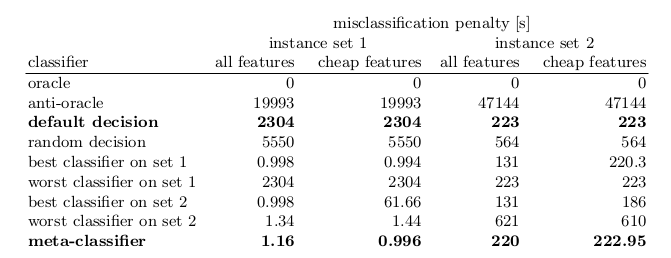
\includegraphics[width=1.0\textwidth]{images/results.png}
  \caption[ ]{Summary of classifier performance on both sets of benchmarks in terms of
total misclassification penalty in seconds.}
  \label{fig:results}
\end{figure}

\begin{figure}[h!]
  \vspace{1 cm}
  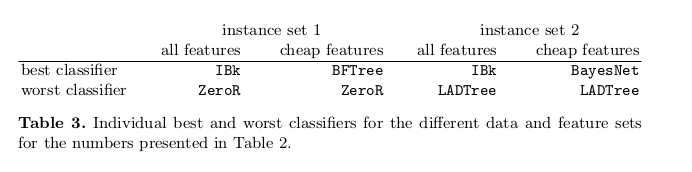
\includegraphics[width=1.0\textwidth]{images/results2.png}
  \caption[ ]{Individual best and worst classifiers for the different data and feature sets.}
  \label{fig2:results}
\end{figure}
